\chapter{Discovery of SARS-CoV-2 main protease inhibitors using synthesis-directed de novo design} \label{ch:ranking}

\begin{quote}
    This chapter is based on Aaron Morris, William McCorkindale, The COVID Moonshot Consortium, Nir Drayman, John D. Chodera, Savaş Tay, Nir London and Alpha A. Lee. Discovery of SARS-CoV-2 main protease inhibitors using a synthesis-directed de novo design model, \textit{Chem. Commun.}, 2021,57, 5909-5912 
\end{quote}

\noindent\hfil\rule{0.5\textwidth}{.4pt}\hfil

% The SARS-CoV-2 main viral protease (Mpro) is an attractive target for antivirals given its distinctiveness from host proteases, essentiality in the viral life cycle and conservation across coronaviridae. We launched the COVID Moonshot initiative to rapidly develop patent-free antivirals with open science and open data. Here we report the use of machine learning for \emph{de novo} design, coupled with synthesis route prediction, in our campaign. We discover novel chemical scaffolds active in biochemical and live virus assays, synthesized with model generated routes.

Coronaviruses are a family of pathogens that is frequently associated with serious and highly infectious human diseases, from the common cold to the SARS-CoV pandemic (2003, 774 deaths, 11\% fatality rate), MERS-CoV pandemic (2012, 858 deaths, 34\% fatality rate) and most recently the COVID-19 pandemic (ongoing pandemic, 1.7 million deaths up to Dec 2020).

The main protease (Mpro) is one of the best characterized drug targets for direct-acting antivirals \cite{pillaiyar2016overview,cannalire2020targeting}. Mpro is essential for viral replication and its binding site is distinct from known human proteases, thus inhibitors are unlikely to be toxic \cite{jin2020structure,liu2020development}. Moreover, the high degree of conservation across different coronaviruses renders Mpro targeting a fruitful avenue towards pan-cornavirus antivirals \cite{ullrich2020sars}. To date, most reported Mpro inhibitors are peptidomimetics, covalent, or both \cite{cannalire2020targeting}. Peptidomimetics are challenging to develop into oral therapeutics, and covalent inhibitors incur additional idiosyncratic toxicity risks. We launched the COVID Moonshot consortium in March 2020, aiming to find oral antivirals against COVID-19 in an open-science, patent-free manner \cite{chodera2020crowdsourcing}.

Here we report the prospective use of algorithmic \emph{de novo} design to rapidly expand hits utilising machine learning (ML) models for ranking compounds by bioactivity as well as synthesis route prediction. Starting from 42 compounds with $\mathrm{IC}_{50}$ within assay dynamic range ($<100 \mu$M) and 515 inactives, our model designed 5 new compounds predicted to have higher activity, together with predicted synthetic routes. All designs were were chemically synthesized and experimentally tested, and 3 have measurable activity against Mpro. The top compound has comparable Mpro inhibition to the best in the training set, but with a different scaffold, and is active against the OC43 coronavirus in a live virus assay.

%Describe GenChem 
% Algorithmic \emph{de novo} design aims to automatically generate compounds that are chemically diverse, synthetically accessible and biologically active \cite{schneider2016novo}. Classic approaches apply heuristics to fragment and modify known active compounds, with the region of chemical space explored and synthetic accessibility constrained by those rules \cite{brown2004graph,patel2009knowledge,hartenfeller2012dogs}. Recent machine learning approaches explore chemical space in more abstract molecular representation space \cite{gomez2018automatic,segler2018generating}, but this often comes at the expense of synthetic accessibility \cite{Gao2020Synthesizability}. Our approach builds on rule-based fragmentation and molecule generation, but employs a method that combines regression and classification amid noisy data, and use of machine learning to predict synthesis routes.

\section{Learning to rank compounds}
Our compound prioritisation model aims to predict whether a designed compound is likely to be an improvement in activity over the incumbent. However, as is typical in the hit-expansion stage, bioactivity modelling is hindered by insufficient data where the majority of compounds are inactive, and noisy data as measurement variability increases for lower affinity compounds. Thresholding the data and framing the problem as classification of active/inactive would not allow us to rank compounds based on predicted improvement over the incumbent, yet the relatively small number of quantitative potency measurement bioactivity data and the measurement noise makes a regression approach challenging.

\begin{figure}[!th]
    \centering
    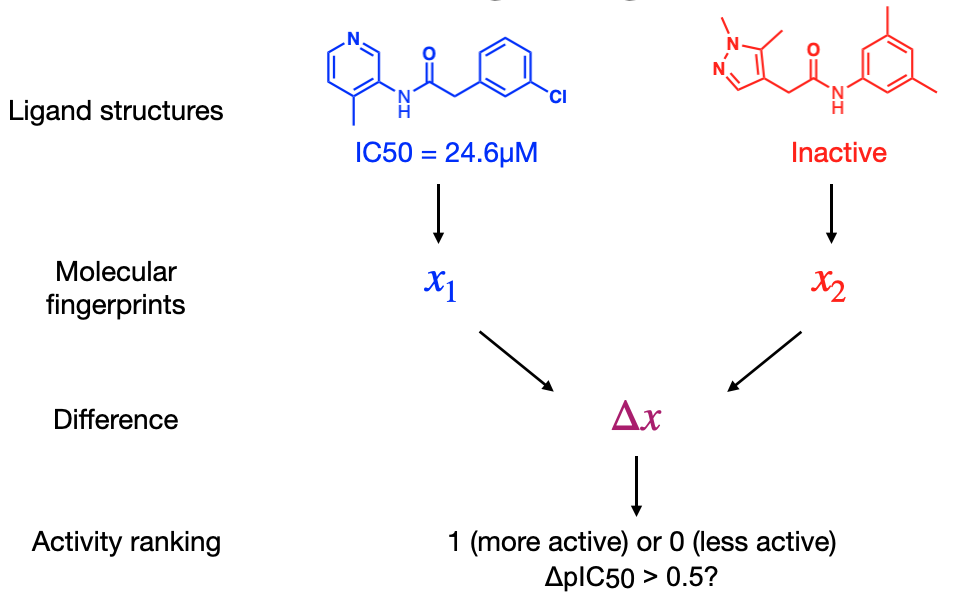
\includegraphics[width=0.85\textwidth]{Chapters/Ranking/Figs/schematic.png}
    \caption{A schematic of the model setup. A classifier takes the difference in molecular fingerprint between two molecules and predicts where one molecule is more or less active than the other.}
    \label{fig:ranking_schematic}
\end{figure}

\begin{figure}[!th]
    \centering
    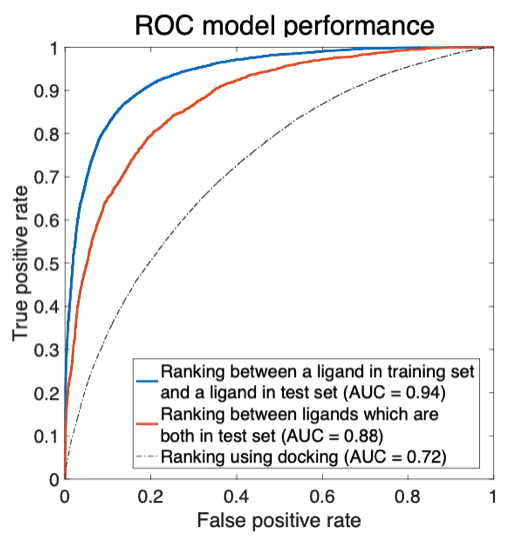
\includegraphics[width=0.65\textwidth]{Chapters/Ranking/Figs/roc_curve.png}
    \caption{Relative ranking of ligands can be predicted by our learning-to-rank machine learning model. The Receiver Operating Characteristic curve of classifying whether a molecule is more/less active than the other.}
    \label{fig:roc_plot}
\end{figure}

Instead of predicting IC50 values directly, we focused our attention on a learn-to-rank approach \cite{duffy2010molecular,agarwal2010ranking} that predicts the pairwise comparison of ligands - given a pair of molecules $(A,B)$, the model predicts whether $A$ is more active than $B$. This approach allows us to assimilate both coarse (active/inactive) and fine (quantitative potency measurements) data into a single model, effectively combining `easy' classification and `difficult' regression into a `moderate' task of ranking input pairs. With a trained ranking model, we can screen for more potent inhibitors by ranking new molecules against the most potent active compounds in the dataset.

To implement this ranking model (Figure \ref{fig:ranking_schematic}), we use the difference in molecular fingerprints between two molecules, $f_A - f_B$ as input to the model, and the output is the whether the molecule $A$ is more or less potent than molecule $B$. The descriptor we use for representing a molecule is a concatenation of 3 512-bit fingerprint representations (Morgan, Atom, Topological Torsion) into one 1536 representation. A multilayer perceptron, implemented via FastAI Tabular framework \cite{howard2018fastai} with default hyperparameters, is used for modelling the data. The choice of molecular descriptor and model was based on empirical performance (Details on the model implementation can be found in Appendix \ref{appendix:ranking}). %The fingerprint is projected onto 20 dimensions using Principal Component Analysis.

To construct a suitable dataset for training the model, the activity data must be reformated into pairs of molecules. This is done by pairing all actives with all inactives, as well as pairing up actives where there is a significant different in bioactivity ($\Delta$pIC50 $>0.5$). This threshold was chosen to match typical assay error, forcing the model to ignore irrelevant experimental noise by ensuring that it is ranking only ligands with demonstrably different bioactivity. The inactive molecules were not paired up between each other as the ranking of inactivity is not relevant to the task at hand and potentially noisy/misleading.

A flipped pairing is included for all pairs so that the dataset is antisymmetric since the model would just predict ones otherwise. Theoretically this method is appealing because it is a natural way of oversampling the low proportion of actives, addressing the problem of dataset imbalance commonly seen in drug discovery classification tasks. Additionally, creating pairs between the actives allows the exploitation of activity information without the noise/difficulty of trying to learn accurate pIC50 values.

% We compare the performance of our model in predicting the pairwise ranking of compounds against the baseline model of simply training a regression model on bioactivities. As a baseline model, we trained a random forest model with the package \texttt{scikit-learn} \cite{scikit-learn}, \texttt{RandomForestRegressor} function, with default hyperparameters. Likewise, for the learning-to-rank model we employ the FastAI tabular model, a general machine learning package for processing classification problems. 

% \begin{table}[]
% \centering
% \begin{tabular}{|l|l|l|}
% \hline
% \textbf{Dataset} & \textbf{RF Baseline AUC} & \textbf{Model AUC}  \\ \hline
% LCK              & \textbf{0.94}              & 0.91          \\ \hline
% opioid           & 0.92                & \textbf{0.94} \\ \hline
% Cannabinoid      & \textbf{0.97}               & 0.87          \\ \hline
% Estrogen         & 0.96               & \textbf{0.98} \\ \hline
% B-raf            & 0.95              & \textbf{0.96} \\ \hline
% Ephrin           & 0.83               & \textbf{0.85} \\ \hline
% Glycogen         & \textbf{0.89}             & 0.88         \\ \hline
% Vanilloid        & \textbf{0.93}              & 0.90          \\ \hline
% JAK2             & 0.97              & \textbf{0.98} \\ \hline
% Dopamine         & 0.97               & \textbf{0.98} \\ \hline
% ABL1             & 0.81               & \textbf{0.84} \\ \hline
% A2a              & 0.58              & \textbf{0.91} \\ \hline
% Coagulation      & 0.82                & \textbf{0.85}  \\ \hline
% Glucocorticoid   & 0.96             & \textbf{0.98} \\ \hline
% Dihydrofolate    & \textbf{0.90}               & 0.86          \\ \hline
% Carbonic         & 0.97              & \textbf{1.00} \\ \hline
% Aurora-A         & 0.89               & \textbf{0.93} \\ \hline
% \end{tabular}
% \caption{Comparing learning-to-rank with direct potency prediction in prioritising compounds.}
% \label{table1}
% \end{table}

For performance evaluation, the dataset was randomly split into training (80\%) and testing (20\%) sets (with roughly the same active/inactive proportion) before the molecules are paired up independently within each set. This ensures that there is no cross-talk between the train/test sets where the model could simply memorize the activity of certain compounds. We train the model on pairs of compounds within the training set and evaluate the model on both pairs within the test set as well as pairs between the training and test set.

Figure \ref{fig:roc_plot} shows that our binary ranking model achieves an AUC of 0.88 (95\% CI: [0.83,0.96]) in ranking ligands within the test set, and AUC for 0.94 (95\% CI: [0.91,0.98]) where we compare a ligand in the training set against another ligand in the test set; the latter is more relevant as our goal is finding ligands more active than the best incumbent. The 95\% confidence interval is computed using bootstrapping. We also compare our model against ranking compounds using docking scores generated with OpenEye's FRED docking algorithm, which achieves an AUC of 0.72 (95\% CI: [0.722,0.723]) (Details of the docking procedure can be found in Appendix \ref{appendix:docking}). Note that docking does not require ligand bioactivity as training data, thus is not a directly comparison to machine learning.

% In the Supplementary Material, we discuss that our model ranks ligands better than a model that directly learns $\mathrm{IC}_{50}$ (AUC = 0.86; 95\% CI: [0.71,0.95]). 

Beyond train-test split, model performance can be evaluated from a time-split. Five months have elapsed from the time we deployed our model for prospective compound selection to writing up the this work. During that time, the COVID Moonshot Consortium (a team of expert medicinal chemists) has independently designed, synthesised and tested 356 compounds \cite{moonshot2020covid}, out of which 15\% were better than the top 2 compounds (having $\mathrm{IC}_{50}$ comparable within error) in our dataset. Table \ref{table:time_split} shows that our model has an enrichment factor of $\sim$2, i.e. if we rescore the 356 compounds synthesized by the medicinal chemistry team using our model, and pick the top 1\%-10\% percentile, the proportion of molecules that would be better than the top 2 compounds would be $\sim$2x higher than human selection. 

\begin{table}[!bh]
    \centering
    \begin{tabular}{|l|l|l|l|}
    \hline
    \textbf{Percentile}        & 1\% & 2.5\% & 10\% \\ \hline
    \textbf{Enrichment Factor} & 1.7 & 2.3   & 1.7  \\ \hline
    \end{tabular}
    \caption{Enrichment factor for the time-split dataset, where we consider model performance on data arriving after the model has been deployed to generate compounds for synthesis and testing. }
    \label{table:time_split}
\end{table}

These retrospective results illustrate that a learning-to-rank approach can leverage bioactivity data from both active and inactive molecules for the enrichment of potent compounds in a real-world drug discovery campaign. In the next section, we deploy our model to discover new Mpro inhibitors in a prospective experiment.

\section{Prospective chemical space exploration}
% Classic approaches apply heuristics to fragment and modify known active compounds, with the region of chemical space explored and synthetic accessibility constrained by those rules \cite{brown2004graph,patel2009knowledge,hartenfeller2012dogs}. Recent machine learning approaches explore chemical space in more abstract molecular representation space \cite{gomez2018automatic,segler2018generating}, but this often comes at the expense of synthetic accessibility \cite{Gao2020Synthesizability}. Our approach builds on rule-based fragmentation and molecule generation,

After designing a well-founded ML scoring model, we must decide on a virtual library of compouds to explore. While one could screen an ultra-large library of make-on-demand compounds as in the previous chapter, it is only feasible for a relatively cheap computational model which is not the case for the ML model developed in this work. 

Instead, we consider a more targeted approach by exploring the chemical space of chemical substructres contained within our initial dataset. Building on rule-based fragmentation methods such as BRICS \cite{Degen2008brics} and CReM \cite{Polishchuk2020Crem}, our general approach is to decompose the existing molecules into a large set of distinct substructure components before enumerating all components with one another, generating a large number of novel and diverse molecules.

\begin{figure}
    \centering
        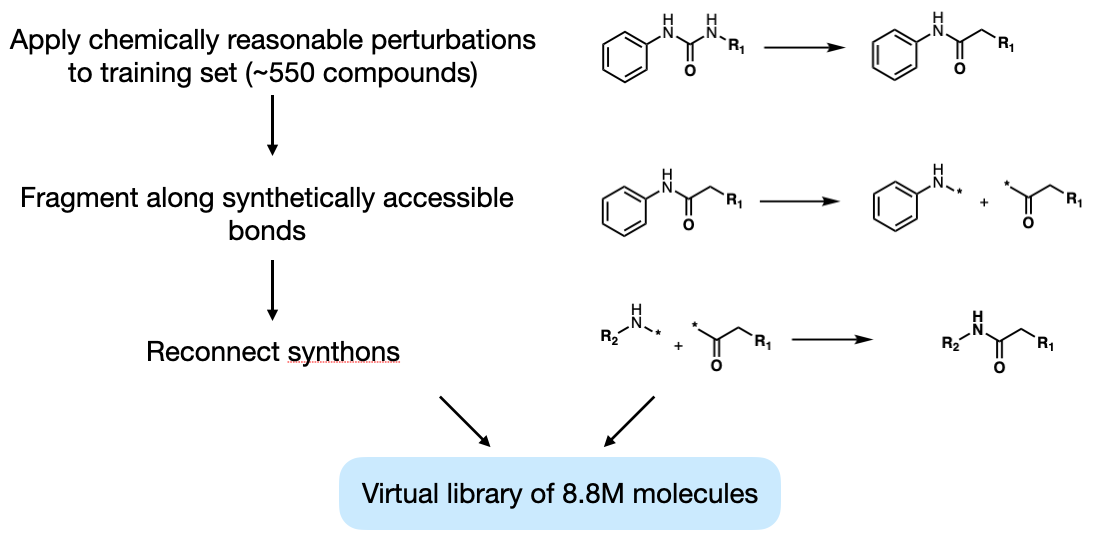
\includegraphics[width=0.75\textwidth]{Chapters/Ranking/Figs/library.png}
        \caption{A schedmatic of the methodology for the library generation process.}
        \label{fig:library}
\end{figure}

Specifically, we first introduce a set of chemically reasonable perturbations (linker and chemotype swaps, e.g. amide to retroamide, amide to urea, swapping N-aryl groups), which is applied to the whole set of active molecules. We then fragment along synthetically accessible bonds (e.g. amides and aromatic C-C and C-N), and reconnect the synthons to generate an exhaustive library (Figure \ref{fig:library}). These operations are defined using SMARTS rules.

The resulting library of 8.8 million generated molecules is then scored against the top 3 compounds in the training set using the learning-to-rank framework, and the mean score is taken as the final score for each compound.

\begin{figure}
    \centering
        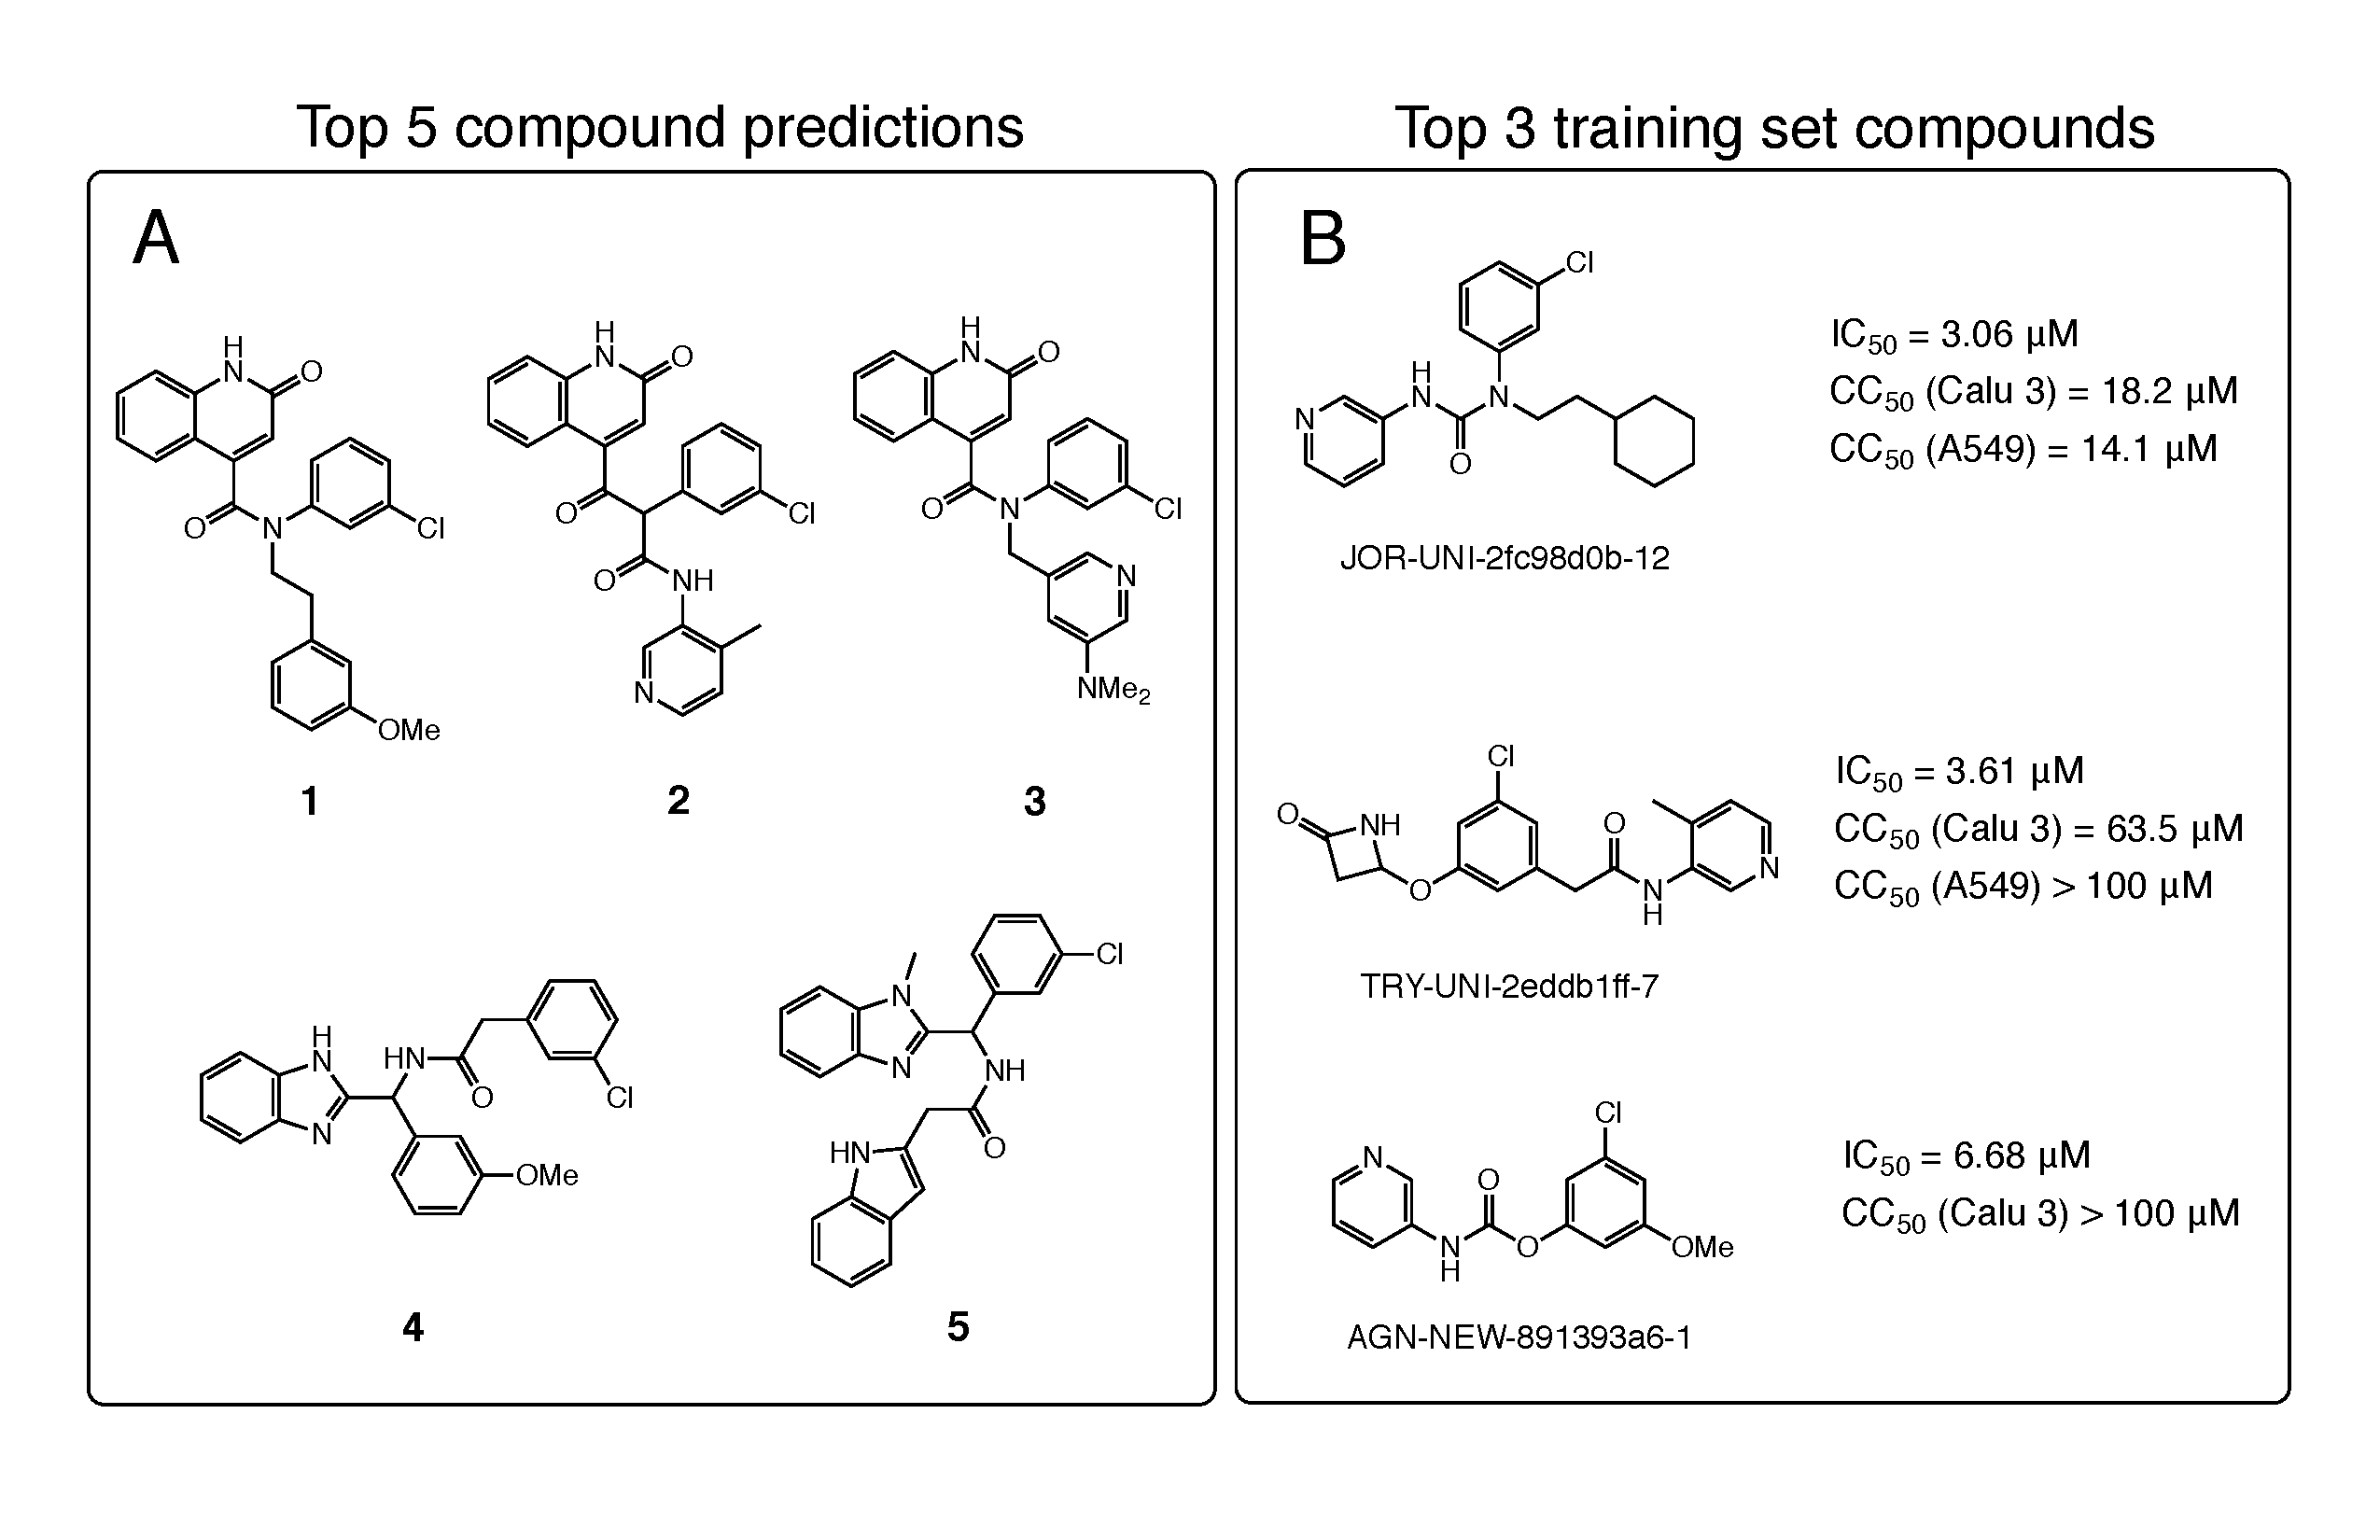
\includegraphics[width=0.75\textwidth]{Chapters/Ranking/Figs/fig2.pdf}
        \caption{Our synthesis-driven design model prioritises molecular scaffold that are not in the top hits. (A) The 5 compounds selected by our methodology for synthesis and testing. (B) The top 3 compounds from the training set, with potency and cytotoxicity measurements.}
        \label{fig:compounds}
\end{figure}

Although virtual ``reactions'' were used to generate new molecules, the synthons are not necessarily off-the-shelf nor the reactions optimal. As such, we use a retrosynthesis predictor to triage based on synthetic accessibility. We used Manifold, a platform for synthesis route prediction (\url{https://postera.ai/manifold}), to generate synthetic routes for the model's top-ranked molecules starting from purchasable building blocks. The underlying technology is based on Molecular Transformer, a machine learning model for reaction prediction using sequence-to-sequence translation \citep{yang2019molecular,schwaller2019molecular}. The top 5 molecules from the screening library with <4 steps in their predicted routes were synthesised and tested (Figure \ref{fig:compounds}A). For comparison, the most potent molecules from the training set are shown in Figure \ref{fig:compounds}B. All five compounds have Tanimoto similarity <0.48 (1024-bit ECFP6) to any molecule in the training set, indicating that the model is not merely reproducing molecules similar to the most potent actives but are exploring novel scaffolds.

\begin{figure}
    \centering
        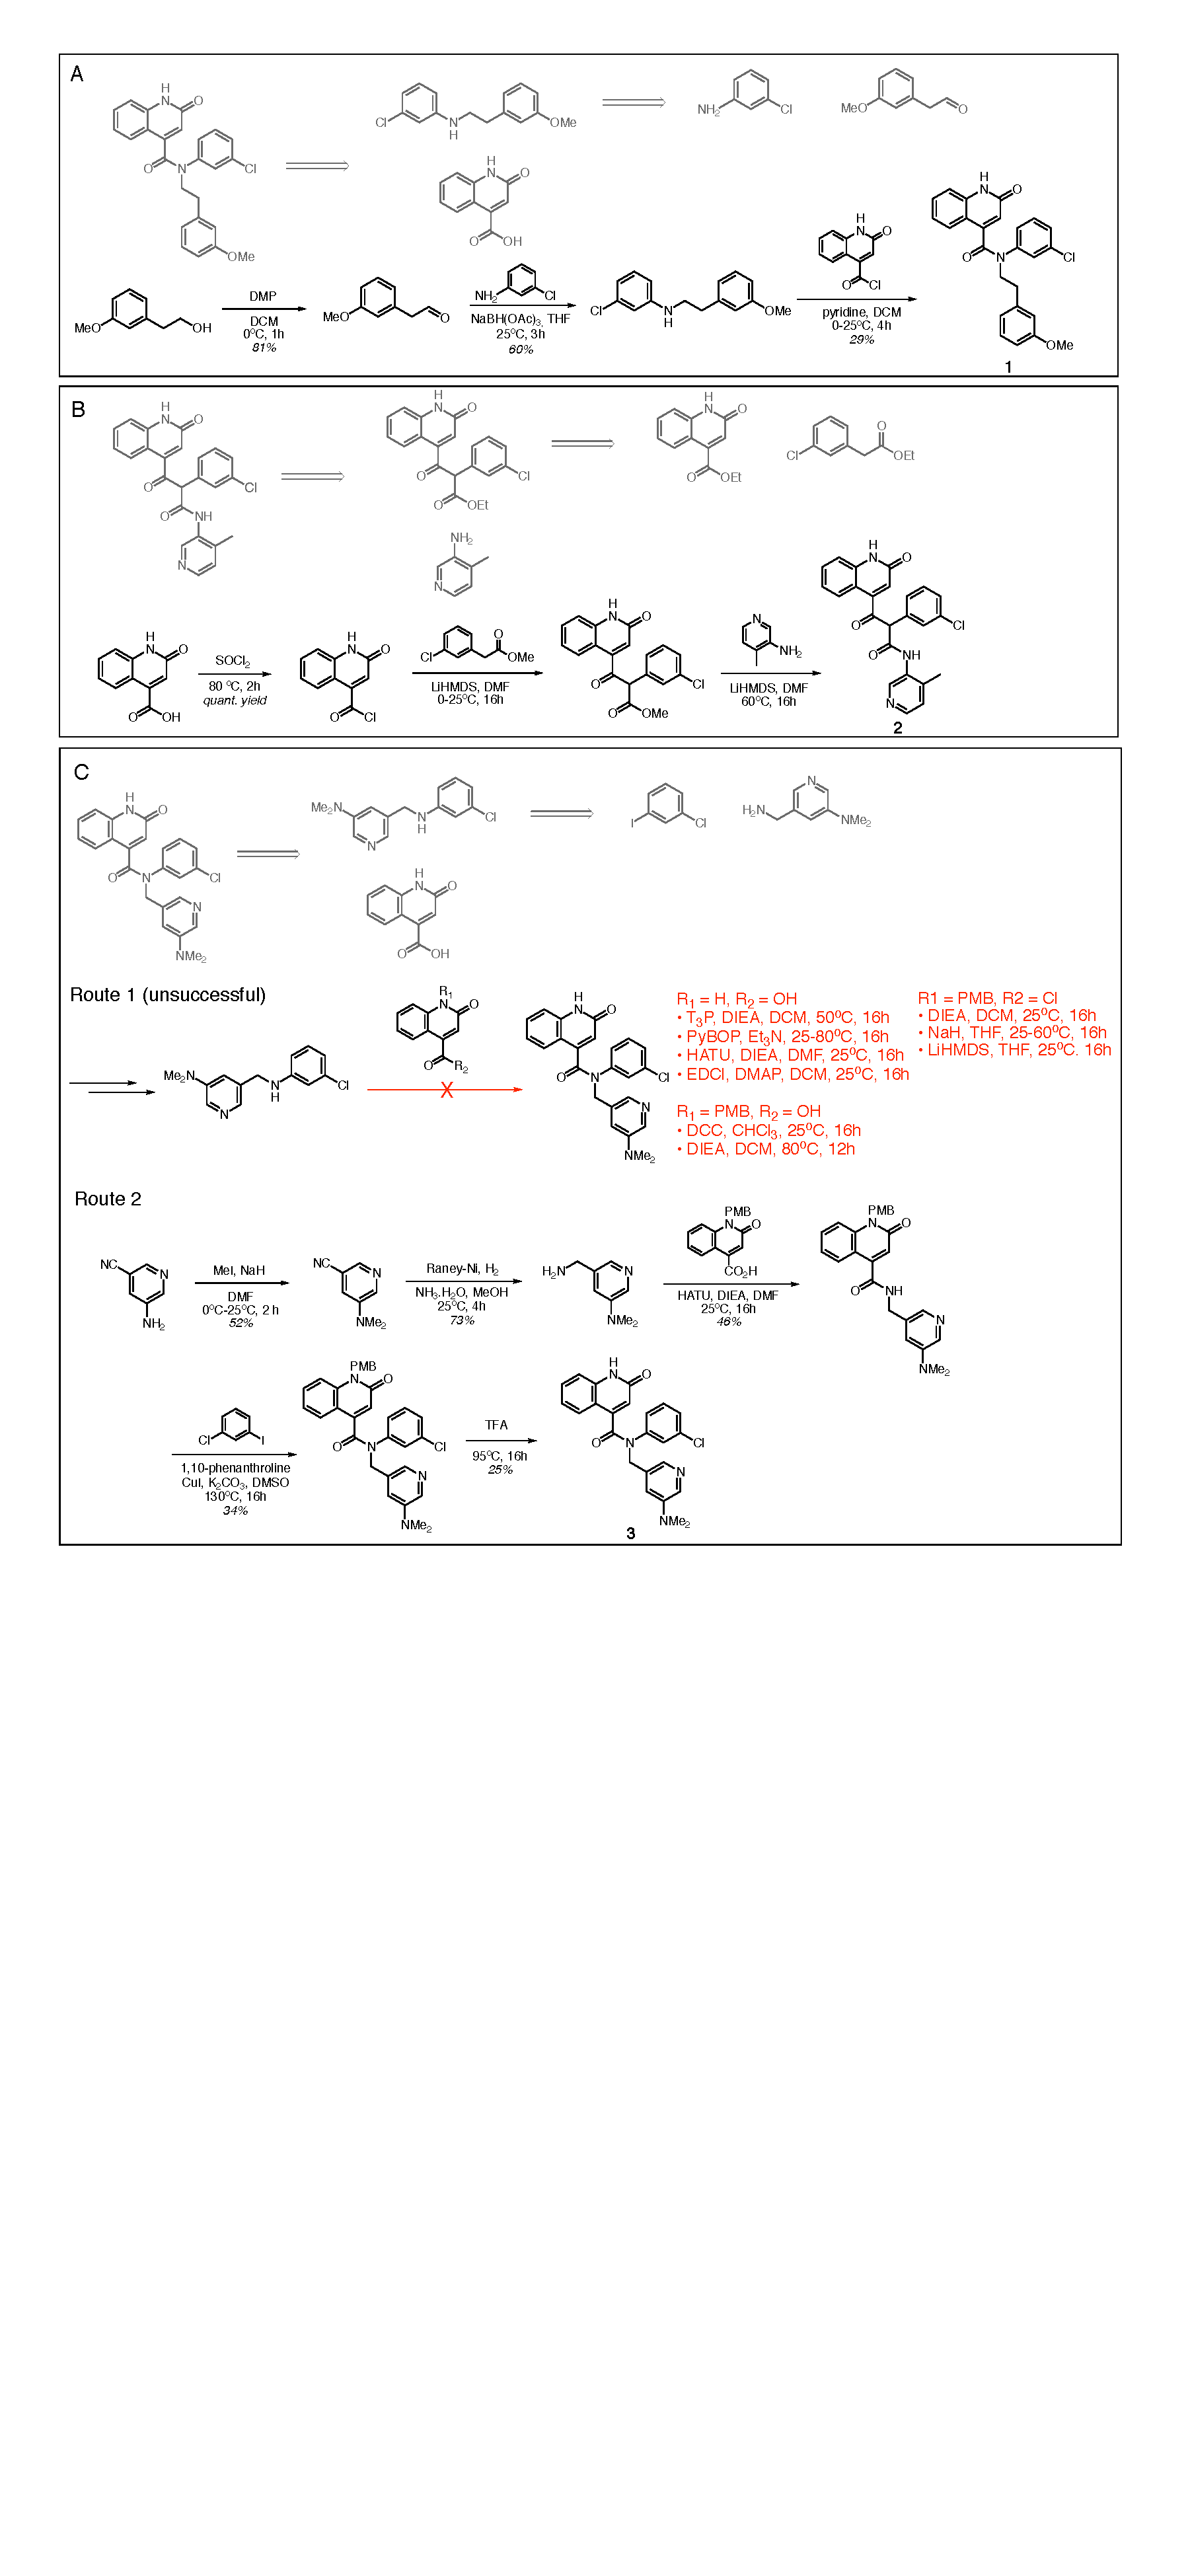
\includegraphics[width=0.65\textwidth]{Chapters/Ranking/Figs/rxn_schemes_1_to_3.pdf}
        \caption{Model generated synthetic schemes that are experimentally validated. Schemes (A)-(C) show the synthesis schemes generated by our model (grey) and experimental schemes (black) for Compounds $\mathbf{1}$-$\mathbf{3}$. The schemes for compounds $\mathbf{4}$ and $\mathbf{5}$ can be found in Appendix \ref{appendix:rxn_schemes}.}
        \label{fig:synthesis_schemes}
    \end{figure}

Figure \ref{fig:synthesis_schemes} shows that for Compounds $\mathbf{1}$, $\mathbf{2}$, $\mathbf{4}$ and $\mathbf{5}$ our retrosynthesis algorithm generates successful routes, thus provides a reasonable estimate of synthetic complexity. The syntheses were carried out at the Wuxi AppTec and compounds were assayed as received. Minor variations in building blocks were employed depending on what was readily available. We note that our algorithm failed to estimate the synthetic complexity of Compound $\mathbf{3}$. The final amide formation step was unexpectedly challenging, and no desired product was seen despite significant efforts in condition screening. Compound $\mathbf{3}$ was furnished via an alternative strategy, employing an Ullmann coupling to arylate the amide, which was not predicted by our approach. 

\begin{figure}[!th]
    \centering
    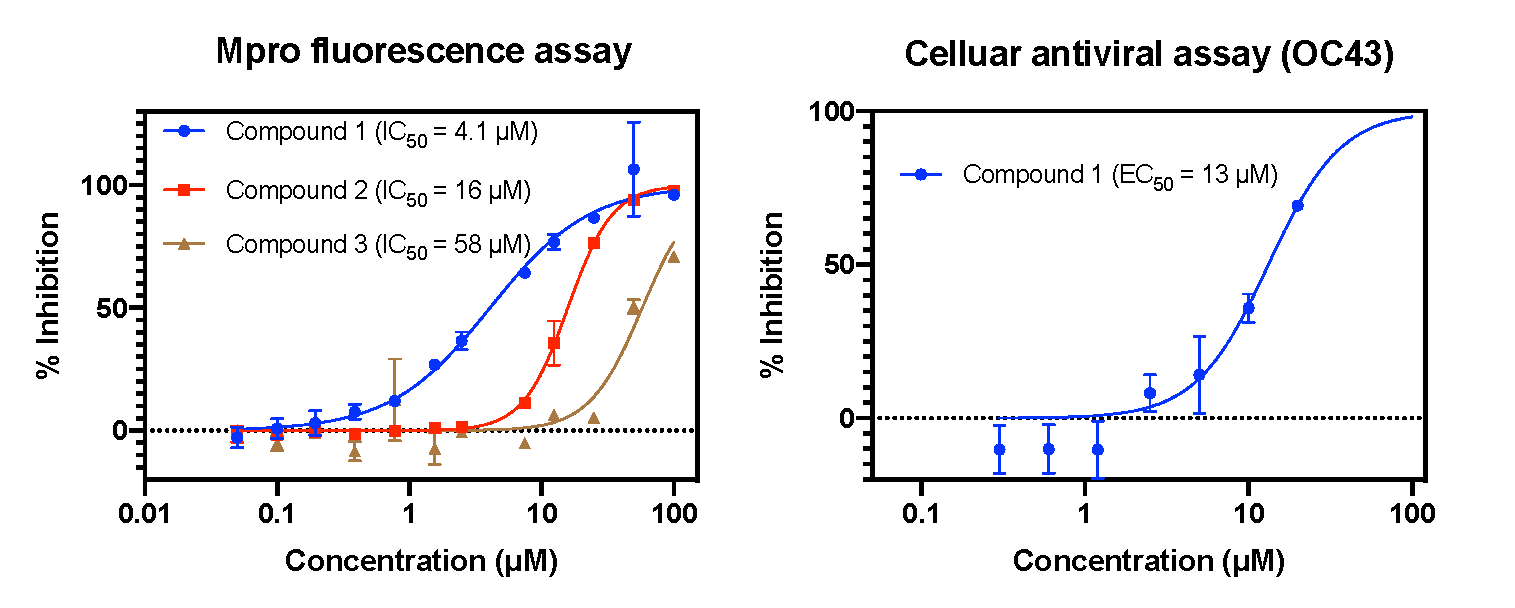
\includegraphics[width=0.85\textwidth]{Chapters/Ranking/Figs/data_curve.pdf}
    \caption{Three compounds generated using our synthesis-directed model exhibit Mpro activity. Our most active compound has measurable antiviral activity against the OC43 coronavirus and no measurable cytotoxic effect.}
    \label{fig:data}
\end{figure}

%result + discussion 
Compounds $\mathbf{1}$-$\mathbf{5}$ were tested for Mpro activity using a fluorescence assay. Figure \ref{fig:data} shows that Compounds $\mathbf{1}$-$\mathbf{3}$ have $\mathrm{IC}_{50}$ within assay dynamic range ($<100 \mu$M), and Compound $\mathbf{1}$ has $\mathrm{IC}_{50} = 4.1 \mu$M (95\% CI: [3.42,4.86]). Compound $\mathbf{1}$ is further assayed in live virus assays, with the less pathogenic OC43 coronavirus, showing $\mathrm{EC}_{50} = 13 \mu$M (95\% CI: [10.1, 18.4]) and is not cytotoxic ($\mathrm{CC}_{50}>100 \mu$M against A549 cell line; $CC_{50}$ is the concentration required to cause 50\% cell death). We employ OC43 as a rapid surrogate assay for SARS-CoV-2 as the former can be done in a BSL-2 rather than BSL-3 lab (See Appendix \ref{appendix:experiments} for assay details). %Interestingly, the top non-cytotoxic hit of the training set (TRY-UNI-2eddb1ff-7) does not show OC43 activity, showcasing the utility of using generative models to suggest new scaffolds with complementary physicochemical properties. 

\section{Discussion} \label{sec:discussion}

In summary, we demonstrated the utility of a \emph{de novo} design framework that learns to rank bioactivity and estimates synthetic complexity, for generating ideas in hit expansion. At the time of writing, optimisation of a quinolone-based scaffold is ongoing in the COVID Moonshot initiative (\url{https://postera.ai/covid}). Data for Compound $\mathbf{1}$-$\mathbf{5}$ is registered as the $\texttt{ALP-POS-ddb41b15}$ series on the Moonshot platform. 

The learning-to-rank approach presented in this chapter is a promising technique for maximally utilising data from inactive compounds as well as accounting for noise in the experimental values. Further work extending this approach to utilise information from ligand-protein complexes has shown great success in hit-to-lead optimisation \cite{Saar2023pnas}. By using docking-based structural descriptors as the input to their ranking model, the authors were able to utilise crystal structures of inactive compounds and outperform docking as well as a fingerprint-based ranking model on ranking ligand activity. Applying this model on a docked structures from a virtual library, the authors were able to greatly improve the potency from their starting point and extended the ligand into unknown regions of the binding site. This result shows the potential for applying ranking-based approaches for modelling bioactivity.

A caveat for pair-based ranking is that even for moderately sized datasets the number of molecular pairs (which is proportional to the square of the dataset size) may become very large and therefore unfeasible to train on. Engineering approaches for efficient sampling of molecular pairs, such as using Tanimoto similarity to constrain pair selection, may be necessary and should be the subject of future work.

% discuss the potential of estimation synthetic complexity for drug design workflows and incorporating it for automated design
The AI-based estimation of synthetic feasibility played a critical role in compound selection in this work and is a promising enabler for automated design workflows in drug discovery \cite{Goldman2022ChemicalDesignLevels}. Beyond the capability to triage libraries by synthesisability and to guide the design of synthetic routes, ML synthesis models could play a key part in an automated drug design workflow. Utilising an automated workflow for the automatic generation of molecular designs as well as decision-making could potentially reduce iteration cycle time, require fewer compounds and iterations to produce a candidate, and scale to more programs \cite{Schneider2018AutomatingDrugDiscovery, Coley2020Outlook}. The framework presented in this chapter is an example of an automated design workflow albeit only with a single iteration - utilisation of multiple iterations via an optimisation \cite{korovina2019chembo} or reinforcement learning feedback loop \cite{born2019paccmannrl} will be a challenging but exciting area of future work.

% \begin{table}[!h]
% \caption{Graph SNN pairwise ranking results}
% \centering
% \label{table:pairwise_table}
% \begin{tabular}{l c c}
% \toprule
%  Series & ROC-AUC & PRC-AUC \\ 
% \midrule
% Chloroacetamides & 0.80 & 0.71  \\

% Acrylamides & 0.78 & 0.80 \\

% Non-covalents & 0.74 & 0.74 \\
% \bottomrule
% \end{tabular}
% \end{table}

% The performance metrics indicate that the model is able to reliably classify whether one compound is more active than another, in particular with much better precision-recall than seen in simply classifying activity.